% THIS IS AN EXAMPLE DOCUMENT FOR VLDB 2012
% based on ACM SIGPROC-SP.TEX VERSION 2.7
% Modified by  Gerald Weber <gerald@cs.auckland.ac.nz>
% Removed the requirement to include *bbl file in here. (AhmetSacan, Sep2012)
% Fixed the equation on page 3 to prevent line overflow. (AhmetSacan, Sep2012)

\documentclass{melta}
\usepackage{graphicx}
\usepackage{balance}  % for  \balance command ON LAST PAGE  (only there!)
\usepackage[utf8]{inputenc}
\usepackage{hyperref}
\usepackage{graphicx}
\usepackage{amsmath}
\usepackage{verbatim}
\usepackage{minted}
\usepackage{listings}
\usepackage{pbox}

\begin{document}

% ****************** TITLE ****************************************

\title{{\ttlit Melta}: Prototipo de una base de objetos en Python 
\titlenote{ \href{https://github.com/bossiernesto/melta}{ODBMS en desarrollo}}}

% possible, but not really needed or used for PVLDB:
%\subtitle{[Extended Abstract]
%\titlenote{A full version of this paper is available as\textit{Author's Guide to Preparing ACM SIG Proceedings Using \LaTeX$2_\epsilon$\ and BibTeX} at \texttt{www.acm.org/eaddress.htm}}}

% ****************** AUTHORS **************************************

% You need the command \numberofauthors to handle the 'placement
% and alignment' of the authors beneath the title.
%
% For aesthetic reasons, we recommend 'three authors at a time'
% i.e. three 'name/affiliation blocks' be placed beneath the title.
%
% NOTE: You are NOT restricted in how many 'rows' of
% "name/affiliations" may appear. We just ask that you restrict
% the number of 'columns' to three.
%
% Because of the available 'opening page real-estate'
% we ask you to refrain from putting more than six authors
% (two rows with three columns) beneath the article title.
% More than six makes the first-page appear very cluttered indeed.
%
% Use the \alignauthor commands to handle the names
% and affiliations for an 'aesthetic maximum' of six authors.
% Add names, affiliations, addresses for
% the seventh etc. author(s) as the argument for the
% \additionalauthors command.
% These 'additional authors' will be output/set for you
% without further effort on your part as the last section in
% the body of your article BEFORE References or any Appendices.

\numberofauthors{1} %  in this sample file, there are a *total*
% of EIGHT authors. SIX appear on the 'first-page' (for formatting
% reasons) and the remaining two appear in the \additionalauthors section.

\author{
% You can go ahead and credit any number of authors here,
% e.g. one 'row of three' or two rows (consisting of one row of three
% and a second row of one, two or three).
%
% The command \alignauthor (no curly braces needed) should
% precede each author name, affiliation/snail-mail address and
% e-mail address. Additionally, tag each line of
% affiliation/address with \affaddr, and tag the
% e-mail address with \email.
%
% 1st. author
\alignauthor
Ernesto Bossi\titlenote{Ing. de la UTN FRBA.}\\
       \affaddr{Universidad Tecnológica Nacional - FRBA}\\
       \affaddr{Medrano 951}\\
       \affaddr{Buenos Aires, Argentina}\\
       \email{bossi.ernestog@gmail.com}
}
% There's nothing stopping you putting the seventh, eighth, etc.
% author on the opening page (as the 'third row') but we ask,
% for aesthetic reasons that you place these 'additional authors'
% in the \additional authors block, viz.

\date{17 de Octubre 2014}
% Just remember to make sure that the TOTAL number of authors
% is the number that will appear on the first page PLUS the
% number that will appear in the \additionalauthors section.


\maketitle

\begin{abstract}
Melta es un prototipo que tiene como objetivo implementar una base de datos orientada a objetos, utilizando el modelo de una propuesta para una nueva estandarización de este tipo de bases de datos \cite{OMG:oodbs}, y haciendo modificaciones y extensiones sobre él. Aportando de esta manera una nueva implementación de este tipo de motores de base de datos en la comunidad.  
\end{abstract}


\section{Introducción}
\label{sec:introduccion}
% Oración muy larga
Con el crecimiento de base de datos no clásicos (base de datos no-SQL), especialmente en el contexto de rápido crecimiento de internet, el problema de procesamiento de datos en sistemas basados en lenguajes orientados a objetos, radica en el procesamiento previo que tienen los datos persistidos desde que se consultan a una base de dato relacional, hasta su transformación en objetos. Estos pasos de procesamiento implican el uso de herramientas, a veces complejas como los ORMs, que son utilizadas para resolver lo que se conoce como \textit{impedance mismatch}\cite{arch:MFowler}.
Las bases de datos orientadas a objetos resuelven estos problemas y presentan otros, tales como la sincronización entre los objetos del dominio o sistema y el de la base de datos. 
En general las bases de datos orientadas a objetos han sido especialmente populares en lenguajes como Smalltalk, en donde los objetos están vivos mientras el sistema esté en ejecución. Esa ventaja permite tener un modelo de objetos a persistir en una etapa intermedia, como lo hace Gemstone. El objetivo de este paper será el de proponer un prototipo para un lenguaje dinámicamente tipado y que pueda extenderse el uso a otros lenguajes, distintos al que se implementó el motor de la base de datos.
% "El lenguaje de implementación [elegido] es Python, ya que.."?
La decisión del lenguaje en el que se implementa dicho prototipo fue Python, ya que permite un rápido modelado del sistema, y se podrán optimizar partes utilizando los bindings de C. 
\\\\
En el futuro se intentará de migrar dicha implementación a otra plataforma que provea mejor soporte para paralelismo, como Jython, o a otro lenguaje, como Scala o Java.
\\\\
El modelo básico de los objetos que se almacenan está basado en una propuesta para una nueva estandarización de bases de datos \cite{OMG:oodbs}. Esta propuesta trata cómo están representados los objetos en la base de datos, y el lenguaje de consulta para interactuar con ella. Mientras los temas tratados son tomados como base, existen otros en los que no se hace hincapié, como la persistencia, y tampoco se define una arquitectura general de como debería ser esta, así como no se hace mención a la transaccionalidad. Estos temas en los que el modelo no hace hincapié se mencionarán a lo largo de este paper.
\\\\
En la sección~\ref{sec:arquitectura} y~\ref{sec:metamodelo}, se tratará la arquitectura principal y el modelo de objetos que existirá en la base de datos. En la sección~\ref{sec:aoql} se profundarizará en el lenguaje de AOQL\@. En la sección~\ref{sec:persistencia} se detallará brevemente la persistencia, en el capítulo~\ref{sec:tran} las transacciones y concurrencia, y en la sección~\ref{sec:conc} las conclusiones y una propuesta de futuras mejoras y nuevas funcionalidades al sistema. 

\section{Arquitectura}
\label{sec:arquitectura}
El modelo de este prototipo es cliente/servidor. El cliente consiste en un módulo que permite la conversión de objetos Python/Melta, un procesador de AOQL, una interfaz que mantiene la relación entre un objeto Python y el id correspondiente en la base de datos, y un conector que permite conectarse con la base de datos. Si bien el formato de los dos tipos de objetos no es el mismo, los objetos de la base de datos tienen conocimiento de la clase a la que pertenece el objeto, su jerarquía, y el estado que tiene. El metamodelo de objetos de Melta se describirá en la sección\ref{sec:metamodelo}.
\\\\
El modelo de objetos que existe en el entorno Python en ejecución, y que está del lado del cliente, tendrá una tabla que relacionará cada objeto que haya sido agregado a la base de datos, con el id del objeto Melta, que existe del lado del servidor. De esta manera se conocerá la relación entre ambos objetos en el cliente y el servidor. Esta relación existe por el tiempo que el entorno del dominio esté en ejecución. Una vez terminada, los objetos que ya no se utilicen en la base de datos y estén presentes en el \textit{schema}, son persistidos y borrados de este, hasta que sean requeridos nuevamente. Como se mencionó previamente, dado que el formato de los objetos del dominio de Python y de Melta no son compatibles, se tendrá un conversor de objetos para hacer el pasaje del estado de los objetos de un lado al otro.
\\\\
El cliente realiza operaciones de consulta y actualización sobre el servidor. Lo puede realizar mediante una interfaz, implementada en el mismo lenguaje que el cliente, o en un lenguaje abstracto llamado AOQL\@. Cuando se requiera de objetos persistidos, se hace una consulta al servidor. En caso de que sea mediante el lenguaje AOQL, la consulta se preprocesa para que luego sea enviada hacia el servidor. Si en cambio se utiliza la interfaz del cliente, este genera el código AOQL correspondiente. Las sentencias se envían al servidor, son recibidas y parseadas por este, y en caso que sean válidas generan operaciones de la API de consulta, que interactúa directamente con la base de datos. De esta manera se restauran aquellos objetos que no estén en el \textit{schema} y que estén involucrados. Luego se devuelve al cliente los objetos o el resultado de dicha operación. Se tratará mas exhaustivamente esto en la sección~\ref{sec:aoql}.
\\\\
El Servidor consiste básicamente en un módulo que escucha nuevas conexiones e intercambia datos con los clientes. Tiene un entorno, llamado \textit{schema}, donde viven los objetos de la base de datos, y un módulo que se encarga de realizar la persistencia y reconstruir las instancias, clases y metadatos del disco al schema, y consecuentemente servirlos al cliente.  
\\\\
El servidor sincroniza las operaciones de lectura/escritura mediante transacciones. Si bien son disparadas por el cliente, el servidor mantiene la información sobre las transacciones que se están llevando a cabo. Se tratará con mas detalle este tema en la sección de concurrencia y transaccionabilidad (sección~\ref{sec:tran}).
% "Otra característica del servidor es que puede persistir.." ?
Otro componente del servidor es el de que pueda persistir o exportar la base de datos completa a otros formatos, tales como json o xml.
\\\\
\begin{figure*}
\centering
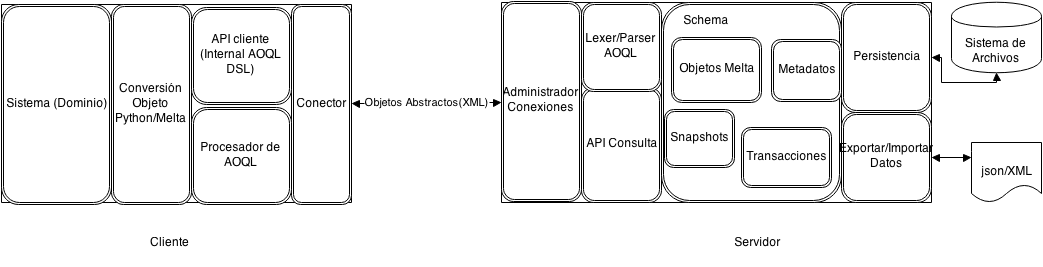
\includegraphics[width=19cm]{MeltaArchitecture}
\caption{Arquitectura General de Melta}
\label{fig:flies}
\end{figure*}

La comunicación entre el cliente y el servidor se realiza, en esta primera versión, serializando los objetos en XML, ya que permite de una manera simple intercambiar instrucciones y objetos entre estos a través de una red de comunicaciones. A pesar de que XML tiene la desventaja de ser demasiado verboso, y que podría utilizarse una librería existente de serialización de objetos, como la librería \textit{pickle} de Python, se optó por XML ya que se desea tener un mecanismo de transporte de los objetos y consultas agnóstico a cualquier lenguaje. En una próxima versión se tratará de implementar un protocolo específico para serializar los objetos y operaciones que el servidor deberá manejar.
\\\\
Con respecto al XML, se presentó el problema de que pueda existir una posible colisión de nombres. Por ejemplo, puede existir una Clase teléfono y una instancia de otra clase que tenga un estado teléfono. Para resolver esto se utilizan los namespaces de XML \cite{xml:BHL06}, que proveen una manera de calificar nombres de atributos y elementos en documentos XML, asociándolos con namespaces identificados por referencias de \textit{Unified Resource Identifier} URI.
\\\\
Con respecto a otras implementaciones, en Smalltalk existe Gemstone y Magma, que poseen una arquitectura similar a la de Melta. Ambas son cliente/servidor, y pueden usarse para almacenar objetos de otros lenguajes como C++, Java y Ruby entre otros. Si bien Melta y Gemstone comparten ciertas similitudes adicionales, como el Schema, y la persistencia con respecto a Magma, el modelo de objetos es diferente en este caso, y está en cambio basado en el estándar de la OMG. Adicionalmente, al ser Melta una base de datos orientadas a objetos minimalista, aún carece de ciertas características que permitan hacer una comparación exhaustiva con otras bases de datos. 

\subsection*{Interacción entre programa y base de datos}

Cuando un programa o aplicación utiliza Melta como base de datos para persistir sus objetos de dominio, la aplicación hace uso del cliente del motor, que se conecta mediante una sesión con el servidor y luego pide la creación de un nuevo schema si es la primera ejecución de la aplicación. En otro caso solo se inicia la sesión explicitando el schema a conectar. Esta interacción hace que el servidor prepare el schema existente en disco.
\\\\
Toda interacción se hace en base a transacciones, y solo se envían los cambios realizados en la aplicación una vez que se hace un \textit{commit} explícito a la sesión. Cuando este evento sucede, se envían los objetos hacia el servidor, que chequea que no haya conflictos de actualidad de los objetos afectados, y los persiste en el schema y en el disco. 
% Tiempos verbales mezclados
Cuando queremos persistir un conjunto de objetos, basta con iniciar una transacción e indicar los objetos que se desea persistir y administrar por Melta. Estos nuevos objetos que se agregaron son enviados al servidor, serializándolos primero en formato XML. Este los deserializa y los agrega al schema. Cuando los objetos son nuevos en un schema, tendrán en su metadata un indicador de que aún son temporales, ya que un \\textit{rollback} haría que estos cambios no se persistieran en disco y se desecharan. Este proceso se realiza porque se debe asignar un nuevo id de objeto por parte del servidor y este notificará al cliente los nuevos ids para los objetos en la cache temporal. Cuando el cliente confirme la operación mediante un \textit{commit}, se envían los cambios realizados desde el cliente al servidor, y si no hay conflictos de concurrencia sobre los objetos modificados, estos se persisten al disco. 
\\\\
Luego de eso, no se necesita mayor interacción con el cliente mas que para mencionar cuando empieza y termina una transacción. 
\\\\
Con respecto a la restauración de los objetos, estos se traen de la base de datos hacia la aplicación mediante consultas en AOQL o por medio de un query builder en el mismo lenguaje que el cliente. Cuando los resultados son brindados por la base de datos estos son convertidos a objetos, de Python en este caso, y agregados a una tabla que relaciona objetos Python/Melta en el cliente. Dicha tabla permite reconocer el objeto que concuerda con el que está en el servidor. Es una tabla de hash y la forma simple de implementarlo es mediante un diccionario. Cuando se consulta sobre objetos que existen en la aplicación, se devuelven objetos clonados de manera shallow al cliente. Cuando se restaura una clase de la base de datos se chequea si existe, y en caso de que alguno de sus métodos sea distinto, se reemplaza el mismo por el que existe actualmente en la base de datos, recompilando ese método dentro de la clase Python. Estos métodos son guardados en formato de \textit{string}. 

\section{Metamodelo de objetos}
\label{sec:metamodelo}
Este paper esta basado en gran parte en el paper de la OMG \cite{OMG:oodbs}, en el que se podrá hacer referencia para conocer más sobre esta sección. El modelo de objetos de Melta se diferencia del de los objetos nativos de Python, en disasociar los objetos con estado en un objeto compuesto, y sus estados como otros objetos atómicos, que pasan a ser inmutables, o sea, ante el cambio, un objeto atómico no se actualiza sino que se crea uno nuevo y se desecha el anterior. Esto permite que pueda darse soporte en el futuro a objetos versionados y facilita la restauración de un estado que esta asociado a una transacción ante un fallo de sincronización o \textit{rollback} de la transacción.
Dichos objetos, poseen un ID,de 128bits de longitud, generado cuando se introduce un objeto en la base de datos por primera vez, y el mismo tiene un formato similar al de UUID, definido en la RFC4122 \cite{UUID:Leach}. Este ID, permitirá identificar unívocamente al objeto en el \textit{schema}, asi como la asociación entre ID de objeto de Python/Melta.
\\\\
\begin{figure}
\centering
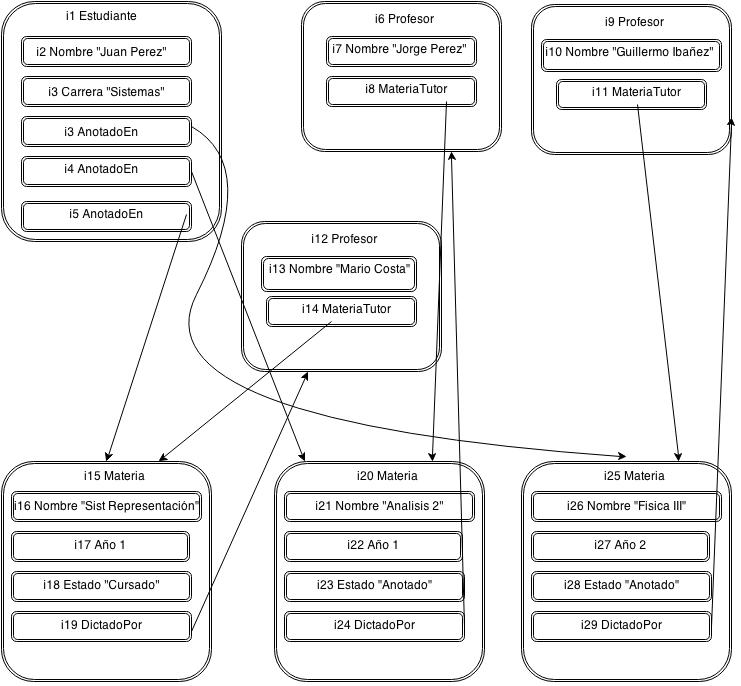
\includegraphics[scale=0.35]{modeloobjetos1}
\caption{Ejemplo de un schema de objetos en Melta.}
\label{melta:modeloObjetos}
\end{figure}

Los objetos que se encontrarán en el \textit{schema} de Melta, en el servidor, serán de estos tres tipos:
\begin{enumerate}
  \item \textbf{Objeto Atómico}: \textit{\textless i,n,v\textgreater} Son objetos, donde i es el ID del objeto, n es el nombre que tendrá el objeto, que será el nombre del atributo de la instancia de Python, y v el valor asociado al objeto. 
  \item \textbf{Objeto Compuesto}: \textit{\textless i,n,T\textgreater} Son objetos donde i es el ID, n el nombre de la instancia de Python y T, una lista de objetos atómicos o de referencia, que componen el objeto.
  \item \textbf{Objeto Referencia}: \textit{\textless i,n,r\textgreater} donde i es el ID del objeto, n el nombre de la instancia referida de Python y r, es el objeto Melta al que se hace referencia. Este tipo de objetos se generan, cuando una instancia tiene en su estado una referencia a otra instancia y representan este estado.
  \item \textbf{Objeto Clase}: \textit{\textless i,c,M,A\textgreater} donde i es el ID del objeto, c es el nombre de la Clase python, M es una lista de métodos que posee la clase y A es una lista ordenada con los ancestros de la clase que se representa en objeto. Las clases poseen invariantes, tales como los métodos de instancia que lo componen, el código que compone cada uno de los métodos, se serializa en un \textit{string} formateado, para respetar en el caso de Python, por ejemplo, la identación. Cuando se desee regenerar la clase nuevamente al levantar el sistema, se evaluarán estos \textit{strings} con el nombre del método almacenado y sus argumentos. Para los métodos de clase, se ha optado por tener un objeto que sea Metaclase.
  \item \textbf{Objeto MetaClase}:  \textit{\textless i,c,C,MC,A\textgreater} donde i es el ID del objeto, c el nombre de la Metaclase Python, C es el objeto clase de la base de datos asociada a dicho objeto Metaclase, MC es una lista de métodos de clase que suministrará al objeto clase C, y A es una lista de los ancestros del objeto Metaclase y son otros objetos Metaclase. Notese que la jerarquía de ancestros de C es la misma que la del objeto en cuestión, solo que el del este último son de objetos metaclase y no de objetos clase (Figura \ref{melta:Metaclase}).  
\end{enumerate}

\begin{figure}
\centering
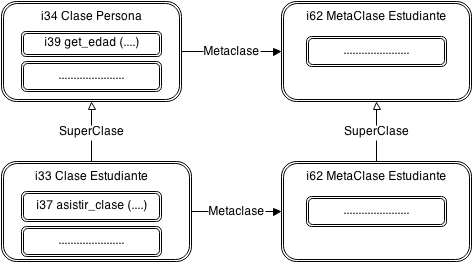
\includegraphics[scale=0.5]{MeltaMetaclase}
\caption{Ejemplo de la jerarquía de clases y metaclases.}
\label{melta:Metaclase}
\end{figure}


Como se menciono en la sección anterior, dichos objetos se encontrarán contenidos en el \textit{schema}, y estos representarán a aquellos objetos que se han recuperado de la base de datos y están en estado de transición durante el tiempo y que pueden variar de acuerdo al flujo del sistema de dominio (Figura \ref{melta:modeloObjetos}). Los objetos que estan en el \textit{schema} estan vivos del lado del servidor, y si bien algunos de estos objetos poseen estado que se relaciona con las invariantes de las clases, no se puede enviar mensajes, al menos en la primera versión del motor.
\\\\
Finalmente, todo objeto posee metadata asociado a el, en donde se define datos tales como la fecha de creación, modificación, si esta asociado a un \textit{schema}, la clase a la que pertenece, y si posee transacciones asociadas, entre otras cosas.

\subsection*{Estructura del Schema}

El \textit{schema}, se compone por todos los objetos y clases que se hayan agregado a la base de datos, y además de eso, soporta lo que es la herencia. En el caso en el que tenemos un objeto de una clase que cambia luego su clase asociada por otro de la misma jerarquía, la base de datos debe evitar una reificación del objeto, descartando el viejo, y creando uno nuevo antes, a partir del estado del anterior, ya que se perdería la identidad del mismo. 
\\\\
\begin{figure}
\centering
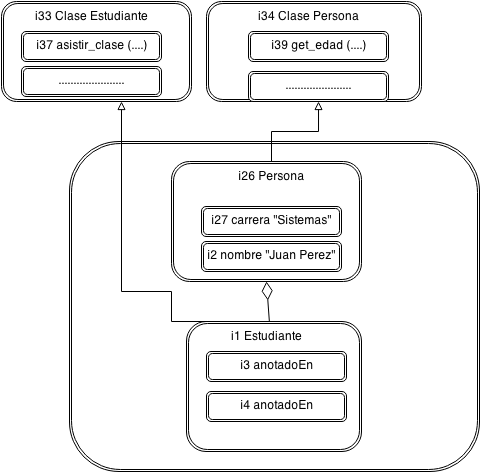
\includegraphics[scale=0.43]{MeltaHerenciaDinamica}
\caption{Herencia dinámica por medio de Roles.}
\label{melta:herenciaDinamica}
\end{figure}

Por ejemplo, si tenemos una clase Persona que define los atributos básicos para una persona pero no para definir un Estudiante, la solución inicial fue la de que Estudiante herede de Persona. Como se menciono antes, si un objeto cambia su clase por otro de la misma jerarquia, es decir, un objeto Persona luego pasa a ser de tipo Estudiante, se crea un nuevo objeto Estudiante a partir del objeto inicial Persona y se desecharía este perdiendo la identidad del objeto. La manera de resolver esto fue mediante composición en donde el objeto Persona tiene el estado propio de su clase y si pasa a ser Estudiante, se crea un objeto de este tipo, solo con el estado propio de la clase Estudiante, y este último objeto se relaciona con el primero mediante una referencia.
\\\\
Utilizando composición se rompe con el principio de sustitución de Liskov \cite{sub:Liskov}, donde cada clase que hereda de otra puede usarse como su padre sin necesidad de conocer las diferencias entre ellas. Formalmente, si S es un subtipo de T, entonces los objetos de tipo T en una aplicación pueden ser sustituidos por objetos de tipo S, sin alterar ninguno de los estados de la aplicación. 

Volviendo al ejemplo, al romperse este principio, no se puede utilizar el objeto Estudiante, cuando se quiera usar el objeto Persona, ya que en este caso, Estudiante no sería más un subtipo de Persona. Esto se resuelve por lo explicado en \cite{OMG:oodbs}, mediante la implementación de herencia dinámica u objetos roles\cite{dynamic:Jodlowski}. Bajo este esquema, una aplicación puede definir subclases a partir de una clase, como en el caso de Estudiante-Persona, y cuando se necesite un objeto del rol Estudiante, el objeto, de la base de datos, de esta clase puede ser creado y ser asociado con el objeto de la superclase y ser disasociado, cuando ya no este actuando en este rol.
\\\\
Ya explicada la herencia del \textit{schema}, se puede definir formalmente al mismo como una tupla \newline \textit{\textless O,C,R,CC,OC,OO \textgreater}, donde O representa a un hash o dicccionario de objetos, del tipo \{i : o\}, donde i es el ID del objeto, y o es la referencia del objeto en si mismo; C es una lista de las clases presentes en el ecosistema, R son los objetos raices del \textit{schema}, estos objetos, son aquellos que pertenecen a instancias de objetos Python. CC es una tabla de hash o dicccionario, del tipo \{c1 : A\}, que relaciona una clase \textit{c1} con su lista de ancestros \textit{A}. OC es un diccionario que relaciona lo que es un objeto con su clase. Notese que CC y OC, son datos que poseen estos objetos en sus respectivas estructuras de metadatos, y solo se vuelven a tener en el \textit{schema}, como tabla maestra. OO define una relación de lo que es la herencia dinámica entre objetos y roles. Por ejemplo si \{i1:i2\} 
\begin{math}
 \in
\end{math} OO, el objeto rol identificado como i1 esta heredado dinámicamente con el objeto identificado como i2. Un ejemplo de esto se ve en la Figura \ref{melta:herenciaDinamica}
\\\\
El \textit{schema}, en la implementación, es un objeto que contiene como atributos a los miembros de la tupla definidos en el parrafo anterior, y que es creado cuando se crear un schema por parte de usuario, o cuando se inicia el motor con dicho schema, y este se genera a partir de lo existente en el disco.
\\\\
Con respecto a lo que es la actualización del sistema, el mismo se resolverá de acuerdo al mecanismo de transacciones, como se mecionó en la sección anterior. 

\begin{figure*}
\centering
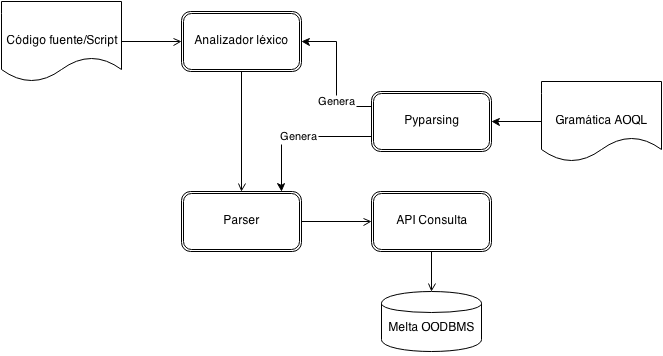
\includegraphics[scale=0.5]{MeltaAOQL}
\caption{Estructura del procesamiento del lenguaje de AOQL.}
\label{melta:aoql}
\end{figure*}


\section{Lenguaje de consulta AOQL}
\label{sec:aoql}

El lenguaje de consulta de AOQL (\textit{Abstract Object Query Language}), es vital para el acceso y persistencia de los datos que utilizará el sistema a lo largo de su ejecución. El mismo podrá ser utilizado en una consola, que actuará como cliente, como en el proyecto en el que se esta utilizando la base de datos. 
Este lenguaje de consulta definirá las operaciones necesarias para el uso de un cliente con la base de datos.
\\\\
Por otra parte el cliente no solo tendrá la posibilidad de comunicarse por medio de un lenguaje de consulta externo, sino que se ofrecerá la posibilidad de que puedan accederse por medio de sentencias en el mismo lenguaje de programación, que el sistema de dominio. De esta manera los programadores podrán hacer consultas sin tener que recurrrir a archivos externos donde esten las consultas, o a tener incluso las mismas mezcladas con el lenguaje de programación concreto del dominio. También se puede ver como no se necesitará de un parser previo para traducir la sintaxis del lenguaje AOQL, a las instrucciones Python propias de la API de consulta, en Python, que consultará a la base de datos.
\\\\
\label{table:gramatica}
\begin{table*}
\centering
\caption{Gramática de AOQL v1}
\begin{tabular}{|c|l|} \hline
Regla gramaticales&Nota\\ \hline
query ::= literal & lista L\\ \hline
query ::= name & lista N\\ \hline
query ::= operadorAlgUnario query& operadores algebráicos unarios\\ \hline
operadorAlgUnario ::= count \mid min \mid sum \mid max \mid - \mid sqrt \mid not \mid avg \mid & \\ \hline
query ::= query operadorAlgBinario query&\\ \hline
operadorAlgBinario ::== \mid< \mid > \mid + \mid - \mid * \mid / \mid and \mid or \mid intersect \mid ...&\\ \hline
query ::= query SinOperadorAlg query& Operador no algebráico.\\ \hline
SinOperadorAlg ::= where \mid . \mid join \mid \forall \mid \exists
query ::= \forall query query \mid \exists query query & Sintáxis alternativa de los identificadores. \\ \hline
query ::= query as name Name& Definición\\ \hline
query ::= query group as name& Agrupamiento\\ \hline
query ::= if query then query& Condicional\\ \hline
query ::= if query then query else query& Otra sintaxis de Condicional\\ \hline
querySeq ::= query \mid query, querySeq& Lista o secuencia de queries\\ \hline
query ::= struct( querySeq ) \mid (querySeq)& Structure constructor\\ \hline
query ::= list( ) \mid list( querySeq )& Constructor de Lista\\ \hline
query ::= set( ) \mid set( querySeq )& Constructor de Set\\ \hline
query ::= (role_name) query & \pbox{20cm}{Casteo dinámico para retornar \\ un rol en particular de un dataSet.} \\ \hline
query ::= query has role role_name& consulta de existencia del rol. \\ \hline
\hline\end{tabular}
\end{table*}

Se puede ver como ambas maneras de acceder a los datos, son coincidentes con lo que son los DSL's (\textit{Domain Specific Language}) externos e internos \cite{dsl:Freeman}\cite{Deursen00domain-specificlanguages:Klint}. En el que el lenguaje AOQL es un DSL externo, que requiere una gramática asociada, ya que es independiente del lenguaje en el que se implementa en la base de datos y el lenguaje en donde existe el sistema que lo utilizará. En cambio las consultas hechas con comandos en un lenguaje de programación, en este caso será Python, ya que se desarrollo el cliente en dicho lenguaje, directamente hará referencia a estas instrucciones del lenguaje AOQL, por lo que este DSL interno, solo será un generador de código de AOQL.
\\\\
Una consulta realizada por un usuario, termina siendo transformada en una sentencia AOQL, que el procesador envia al servidor, por medio de conector, mediante un simple contector, en la implementación un socket, donde se envían las consultas en formato de string, y al llegar al servidor, este las procesará mediante un analizador léxico y un \textit{parser}, que puedan procesar el lenguaje y traducirlo a instrucciones de la API de consulta (figura \ref{melta:aoql}). Esta API de consulta, hara los requerimientos a la base de datos, y una vez que se obtengan los objetos resultantes, estos se agruparán en una lista, se serializarán en formato XML y se devolverán al cliente. 
\\\\
A continuación se presentan algunos ejemplos de como se interactua con ambos DSL's desde una aplicación en Python. Se comienza siempre utilizando un query builder, que permite realizar consultas por medio del DSL interno o externo, y se deja el uso a prefernecia del usuario.

\begin{minted}[mathescape,
               linenos,
               numbersep=5pt,
               gobble=2,
               frame=lines,
               framesep=2mm]{Python}
  
  session = MeltaSession(host='localhost',
  schema='Universidad')
  query = MeltaQueryBuilder(session)
  
  #Sentencia AOQL
  query.aoql_sentence('Estudiante all')

  #Sentencia por query builder
  query.type(Estudiante).all()
  #Devuelve un resultset con la lista de los objetos
  #resultantes
  query.send() 


  #Ejemplo con condicion
  #Sentencia AOQL
  query.aoql_sentence('Estudiante where (id > 2000)')

  #Sentencia por query builder
  #En el futuro estaria bueno cambiar el where por un
  #find con un lambda -> 
  #query().table(Estudiante,e).find(lambda e: e.id > 2000) 
  query.type(Estudiante).where(value.Greater('id',2000))
  query.send()

  #Ejemplo con seleccion de atributos
  #Sentencia AOQL
  query.aoql_sentence('Estudiante where (id > 2000)')

  #Sentencia por query builder
  query.type(Estudiante).where(value.Greater('id',2000))
  .return('nombre', 'anotadoEn.nombre_materia')
  query.send() #devuelve un ResultSet 

  #Ejemplo de Rol
  #Sentencia AOQL
  query.aoql_sentence('(Persona) Estudiante 
  'where (nombre == "Juan")')
  
  #Sentencia por query builder
  query.type(Estudiante).where(value.Eq('nombre','John'))
  .asRole('Persona')
  query.send() #devuelve un ResultSet de Personas

\end{minted}

En un futuro debería definirse un pequeño motor de optimización de consultas para minimizar la cantidad de operaciones hacia el servidor y de esta manera tener un menor tiempo de espera, en obtener datos o resultados por parte del cliente.

\subsection*{Gramática del lenguaje AOQL}

El lenguaje de AOQL, en su primera versión estará conformada por la gramática descripta en la tabla 1.
\\\\
Dicha tabla estaba basada en el trabajo en \cite{OMG:oodbs}, con algunas pequeñas modificaciones, como la eliminación de bags y se agrego el tipo Set a la gramática. En el futuro, se podría pensar una extensión de los tipos de colecciones para soportar otros lenguajes de programación que hagan uso de este motor. En cuanto a la implementación, se implemento el lenguaje utilizando una herramienta que permite generar un analizador léxico y un \textit{parser} a partir de la gramática definida en la tabla \cite{Comp:AhoSethiUllman}. Luego de eso, se armo un intérprete directo que hace uso de la API de consulta contra la base de datos.

\section{Persistencia}
\label{sec:persistencia}
Melta posee un modulo de persistencia en donde se almacenan físicamente los objetos pertenecientes al \textit{schema}, una vez que se haya hecho un \textit{commit} en la transacción. En la primera versión solamente se persisten los cambios detectados en el sistema hacia el \textit{schema}, solo cuando esto suceda. La arquitectura básica de los formatos de base de datos en disco está basada en el de la base de datos Magma. \cite{magma:gaylard}
\\\\
Como se trato previamente en el documento, los objetos en Melta están identificados por un identificador único. Este identificador unívoco se utiliza en el archivo donde se almacenan a aquellos objetos que no estén siendo utilizados durante la ejecución. Cuando se solicite un objeto, por parte de un cliente, que no exista actualmente en el schema, se procede a leerlo del archivo en donde esta almacenado, y un módulo de extracción convertirá el objeto en disco en formato Melta, asimismo, se extrae la metadata del mismo que también esta serializado. Cuando se reconstruye el objeto, se chequea si la clase o rol que tiene asociado actualmente existe en el \textit{schema}, si no existe se trae el mismo también. Actualmente si un objeto que se reconstruye del disco posee referencias actuales a un objeto referencia, se reconstruye este y el objeto original de manera \textit{eager}. O sea que ante un objeto que posee una referencia hacia otro objeto, el módulo de restauración traerá ambos de la base de datos y también si alguno de los dos objetos es el primero de su tipo en ser incorporado al schema, se traerá su clase y metaclase correspondiente.
\\\\
Con respecto al formato del archivo, actualmente esta en desarrollo, pero se tiene una primera versión del mismo, con una arquitectura, en la que la persistencia de un \textit{schema}, se haga en dos archivos separados, el primero es de extensión .mlt, donde se almacenan todos los objetos pertenecientes al \textit{schema}, una vez que se transaccione, el mismo esta compuesto por una cabecera de 8192 bytes, que contiene una \textit{binary signature}, que procura la integridad de los datos a cierto punto (esto depende del algoritmo que se emplee para este propósito), un número de versión, la metadata propia del \textit{schema}, cantidad de objetos persistidos, el tamaño del archivo total, una lista de punteros libres, y el puntero inicial donde comienza el primer objeto. Luego se tiene un directorio, donde esta el puntero de cada uno de los objetos que conforman el archivo. 

\begin{figure}
\centering
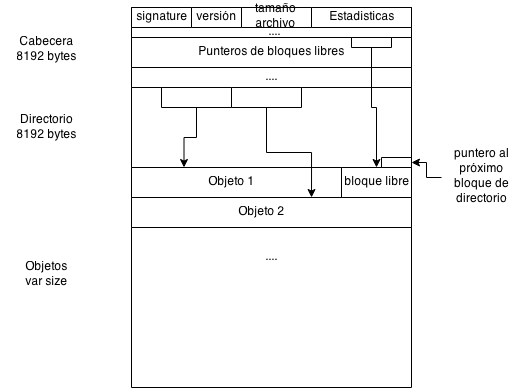
\includegraphics[scale=0.5]{meltafileformat}
\caption{Estructura del tipo de archivos .mlt .}
\label{melta:mltformat}
\end{figure}

El mismo es de una longitud fija de 8192 bytes, y en caso de que se supere dicho límite, siempre se tiene una referencia al próximo bloque del directorio, y de esta manera, se comporta como una lista secuencial de bloques. 
\\\\
Luego del directorio se tienen los objetos, de longitud variable, de acuerdo a lo que ocupen, cuando se agrega un nuevo objeto se agrega al final del archivo, y cuando se elimina uno, se libera el bloque del disco, y se agrega el puntero a la lista de punteros libres. El problema que existe es análogo al que sucede con un asignador de memoria, en el que aumenta la fragmentación a medida que pase el tiempo, para remediar esto, en primera medida, cada X (este valor es configurable) veces que se monte el filesystem, cuando se inicializa la base de datos, se compacta el archivo y se actualiza el directorio. Una mejora a esto sería que en vez de agregar siempre al final se tenga un algoritmo de first-fit, y de esta manera se reduzca el espacio libre fragmentado, sin embargo, se debe hacer una compactación luego de un tiempo.\ref{melta:mltformat}
\\\\
El segundo archivo contiene los datos de indexación de los objetos, y este archivo se levanta en su totalidad cuando se inicialice el motor de base de datos, su objetivo es obtener rápidamente los objetos a restaurar por clase, y la reindexación la maneja automáticamente el modulo de persistencia y recuperación. Este archivo solo se persiste cuando se guardan los cambios en la base de datos, y al estar levantado todo el índice en memoria, no existe fragmentación.
\\\\
Finalmente cuando una transacción global sea exitosa, se guardan los cambios en el \textit{schema}, consecuentemente hay una manera de decir al sistema de que se desean persistir en disco lo que existe actualmente en el \textit{schema}, y es mediante un comando llamado snapshopt, que persiste los cambios en el disco. 

\begin{figure*}
\centering
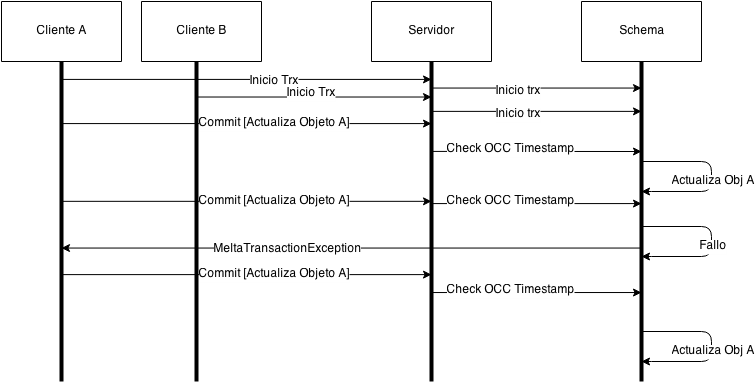
\includegraphics[scale=0.5]{Transaccion}
\caption{Ejemplo del Optimistic Concurrency Control.}
\label{melta:occ}
\end{figure*}

\newpage
\section{Transacciones y Concurrencia}
\label{sec:tran}
Melta soporta modificaciones concurrentes de objetos, por varios clientes que esten conectado al servidor, toda modficiación, del lado del cliente debe estar enmarcado en una transacción, esto provee dos características importantes:

\begin{itemize}
\item \textbf{Atomicidad}: Las transacciones son exitosas o falla, y al ser transacciones, no hay estado que se mantenga hasta que se haga \textit{commit} a una transacción.
\item \textbf{Control de Concurrencia}: las transacciones se ejecutan como si tuviesen acceso exlusivo a los datos, de esta manera, multiples transacciones pueden correr concurrentemente y de esta manera la lógica de la aplicacion no tiene que tomar en cuenta el acceso concurrente.
\end{itemize}

Las transacciones utilizan el principio de \textit{Optimistic Concurrency Control}, mediante un timestamp. Los cambios que se hacen a uno o más objetos mientras los cambios no esten aplicados, mediante un \textit{commit}, son realizado de manera independiente y del lado del cliente, que mantendrá sus objetos modificados en una cache, y de esta manera no tiene que ser bloqueados, los cambios recien se sincronizarán cuando el cliente haga un \textit{commit} explicito. Solo se permite que una transacción aplique los cambios en un momento determinado. Si hay dos threads, o clientes, que modifican un el mismo objeto, uno de ellos aplicará los cambios primero. Cuando el segundo aplique los cambios, el cambio que aplique será inválido y se le retornará una excepción al mismo. El dominio o aplicación debería atrapar esta excepción y ejecutar de nuevo la aplicación de los cambios, cuando esto suceda, los estados de los objetos afectados, reflejan cambios hechos por las transacciones ya exitosas en el servidor.

\section{Conclusiones}
\label{sec:conc}
Si bien este paper es una versión temprana de un prototipo de una base orientada a objetos, en esta primera versión se definió una primera aproximación de una arquitectura para un model cliente/servidor básico. Los próximos objetivos, para tener un prototipo más completo, son los siguientes:

\begin{itemize}
\item Proponer un protocolo para comunicación de objetos serializados y operaciones entre cliente/servidor ya que el pasaje de consultas y objetos se hace por XML y resulta demasiado verboso.
\item Objetos versionados.
\item Replicación.
\item Bases de datos distribuidas que conformen un ambiente \cite{ODRA:sub}.
\item Optimización del Motor y de sentencias AOQL.
\item Acceso cruzado a otras bases de datos orientas a objetos.
\item Seguridad: Securitizar comunicaciones entre cliente/servidor, y proveer mecanismos de permisos para restringir acceso de la base de datos a usuarios.
\item Tolerancia a fallos, por interrupción del servicio causado por fallas electricas o de red.
\end{itemize}
%\end{document}  % This is where a 'short' article might terminate

Actualmente se esta desarrollando una implementación de este protoripo, como se mencionó en la introducción, y el objetivo es implementar la arquitectura propuesta en este documento. Los siguientes pasos involucrarían la optimización del motor y de testear el mismo con una mayor carga de datos a fin de evaluar si es viable el uso de este motor en ambientes productivos. 
Si bien algunas de las partes, como el metamodelo son basadas fuertemente en \cite{OMG:oodbs}, se hicieron algunas modificaciones sobre este, y se diseño una arquitectura simple para una primera versión de este motor de base de datos. 


% ensure same length columns on last page (might need two sub-sequent latex runs)
\balance

%ACKNOWLEDGMENTS are optional
\section{Agradecimientos}
Agradecimientos en especial a la OMG, por su propuesta de un nuevo estandar, que me dio el interés para investigar y desarrollar este prototípo en esta tecnología emergente.

\nocite{*} 
% The following two commands are all you need in the
% initial runs of your .tex file to
% produce the bibliography for the citations in your paper.
\bibliographystyle{abbrv}
\bibliography{melta_blib}  % vldb_sample.bib is the name of the Bibliography in this case
% You must have a proper ".bib" file
%  and remember to run:
% latex bibtex latex latex
% to resolve all references

%APPENDIX is optional.
% ****************** APPENDIX **************************************
% Example of an appendix; typically would start on a new page
%pagebreak

%\begin{appendix}

%\end{appendix}



\end{document}
